%=====================================================================
%  Physics of Learning  --  Chapter 4
%  The Replica Method I: A Single-Spin Toy Model
%  Style: tufte-handout.   Compile with pdflatex (x2 for refs).
%=====================================================================
\documentclass[nobib,justified]{tufte-handout}

\usepackage{amsmath,amssymb,mathtools}
\usepackage{tikz}
\usetikzlibrary{arrows.meta,positioning,calc}
\usepackage{pgfplots}
\pgfplotsset{compat=1.18}
\usepackage{microtype}

% ---- title ----------------------------------------------------------
\title{The Replica Method I:\\ A Single-Spin Toy Model}
\author{Physics of Learning \textbullet\ IIT Madras}
\date{}

% ---- helpers --------------------------------------------------------
\newcommand{\dbar}[1]{\overline{#1}}            % disorder average
\newcommand{\Dz}{\mathcal{D}z}                   % gaussian measure
\definecolor{spinup}{HTML}{2E7D55}
\definecolor{spindown}{HTML}{B3412B}
\definecolor{accent}{HTML}{2A6FA8}

% boxed key result
\usepackage[most]{tcolorbox}
\newtcolorbox{keyresult}{
  enhanced, colback=accent!6, colframe=accent!75!black,
  boxrule=0.6pt, arc=2pt, left=6pt,right=6pt,top=4pt,bottom=4pt,
  before skip=8pt, after skip=8pt}

% small spin arrows for inline / margin use
\newcommand{\spinup}[1][1]{\tikz[baseline=-0.6ex]{\draw[spinup,line width=1.3pt,-{Stealth[length=2.4mm]}](0,-0.28)--(0,0.36);}}
\newcommand{\spindown}[1][1]{\tikz[baseline=-0.6ex]{\draw[spindown,line width=1.3pt,-{Stealth[length=2.4mm]}](0,0.36)--(0,-0.28);}}

\begin{document}
\maketitle
\noindent{\itshape\large Chapter 4}\vspace{4pt}\hrule\vspace{10pt}

\begin{abstract}
\noindent
We introduce the replica method---the central technique for computing
disorder-averaged free energies in disordered systems and in the
statistical mechanics of learning. The whole conceptual apparatus is
developed on the simplest nontrivial example: a single binary neuron
in a random field. Every intermediate step is shown. By the end we have
computed $\dbar{\ln Z}$ two independent ways (validating the method) and
learned to \emph{read} the free energy as a statement about how strongly
data determines a neuron. This chapter is the conceptual scaffold for
Chapter~5, where the same steps---applied to a system of $N$ coupled
spins---produce genuine phase transitions in learning.
\end{abstract}

%---------------------------------------------------------------------
\section{Why we must average a logarithm}

\newthought{In a learning problem} the data, or the couplings built from
it, are random but \emph{fixed} for a given task.\sidenote{This is called
\emph{quenched} disorder, as opposed to \emph{annealed} disorder which
fluctuates on the same timescale as the degrees of freedom. The
distinction is the whole reason the replica method is needed.}
For one such fixed sample, the thermodynamics is governed by the free
energy
\[
  F = -\frac{1}{\beta}\ln Z, \qquad
  Z = \sum_{\{\mathbf s\}} e^{-\beta H[\mathbf s]}, \qquad \beta = \frac1T .
\]
Physical observables are \emph{self-averaging}: a large system behaves
like the typical sample, i.e.\ like the average over disorder. The object
we actually need is therefore the disorder-averaged free energy
\[
  \dbar{F} = -\frac{1}{\beta}\,\dbar{\ln Z},
\]
where $\dbar{(\cdot)}$ denotes the average over the quenched randomness.

\newthought{Here is the difficulty.} Averaging $Z$ itself over disorder is
typically easy---it is a Gaussian integral. But averaging $\ln Z$ is hard:
the logarithm entangles the disorder with the thermal sum in a way that
refuses to factorise. The replica method is the standard device for
circumventing exactly this obstruction.

%---------------------------------------------------------------------
\section{The replica identity}

The escape hatch is an elementary algebraic identity:
\begin{keyresult}
\[
  \ln Z = \lim_{n\to 0}\frac{Z^{\,n}-1}{n}.
\]
\end{keyresult}
\noindent
\textbf{Verification.} Expand $Z^n = e^{n\ln Z} = 1 + n\ln Z + O(n^2)$.
Then $(Z^n-1)/n = \ln Z + O(n) \to \ln Z$ as $n\to 0$. \hfill$\square$

\medskip
Averaging both sides converts the hard object into
\[
  \dbar{\ln Z} = \lim_{n\to 0}\frac{\dbar{Z^{\,n}}-1}{n}.
\]
The point is that $\dbar{Z^n}$---the average of the $n$-th
\emph{power}---is computable. For integer $n$, $Z^n$ is simply $n$
identical, independent copies (``replicas'') of the system:
\[
  Z^n = \underbrace{Z\cdot Z\cdots Z}_{n}
      = \sum_{\{s^1\}}\!\cdots\!\sum_{\{s^n\}}
        e^{-\beta\sum_{a=1}^n H[s^a]}.
\]
The replicas $s^1,\dots,s^n$ are identical copies that \emph{share the
same disorder}. When we average over that shared randomness, it couples
the replicas together---and that coupling is the entire mechanism.

\newthought{The sleight of hand} is this: we compute $\dbar{Z^n}$ for
\emph{integer} $n$, obtain a formula, then \emph{analytically continue} it
to real $n$ and send $n\to 0$.\sidenote{This continuation is the
mathematically delicate step. In this chapter it is completely harmless;
in Chapter~5 it becomes the subtle heart of the method.}

%---------------------------------------------------------------------
\section{The toy model: one neuron in a random field}

\marginnote{%
\centering
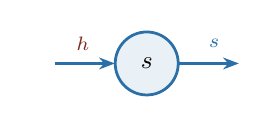
\begin{tikzpicture}[scale=0.9]
  \draw[accent,line width=1pt,-{Stealth[length=2mm]}] (-1.3,0)--(-0.45,0);
  \node[circle,draw=accent,line width=1pt,fill=accent!10,minimum size=8mm]
       (n) at (0,0) {\small$s$};
  \draw[accent,line width=1pt,-{Stealth[length=2mm]}] (0.45,0)--(1.3,0);
  \node[spindown] at (-1.55,0) {};
  \node[font=\scriptsize,spindown!70!black] at (-0.9,0.28) {$h$};
  \node[font=\scriptsize,accent] at (0.95,0.28) {$s$};
\end{tikzpicture}\\[2pt]
\footnotesize A single neuron $s=\pm1$ driven by a random field $h$.
}

Take a \emph{single} spin $s=\pm1$ in a random field $h$, where $h$ is
Gaussian with zero mean and variance $\sigma^2$:
\begin{keyresult}
\[
  H[s] = -\,h\,s, \qquad s = \pm 1, \qquad h \sim \mathcal N(0,\sigma^2).
\]
\end{keyresult}
\noindent
Interpret $s=+1$ (\spinup) as the neuron \emph{firing} and $s=-1$
(\spindown) as \emph{silent}. The field $h$ is a random input or bias---it
plays the role of the quenched disorder, ``the data.'' The energy $-hs$ is
lowest when $s$ aligns with $\operatorname{sign}(h)$: the neuron tries to
match its input.

\medskip
For a fixed field $h$ the partition function is immediate:
\[
  Z = \sum_{s=\pm1} e^{\beta h s}
    = e^{\beta h} + e^{-\beta h}
    = 2\cosh(\beta h).
\]
Our goal is the disorder average $\dbar{\ln Z}$, with the average taken
over $h$.

%---------------------------------------------------------------------
\section{The direct route (our ground truth)}

Because this model is so simple, we can average the logarithm directly:
\begin{equation}\label{eq:direct}
  \dbar{\ln Z}
  = \int_{-\infty}^{\infty}\frac{dh}{\sqrt{2\pi\sigma^2}}\,
    e^{-h^2/2\sigma^2}\,\ln\!\big(2\cosh\beta h\big).
\end{equation}
This is a perfectly good one-dimensional integral. We keep
Eq.~\eqref{eq:direct} in reserve: at the end we will reproduce it via
replicas, confirming the method on a case where we already know the answer.

%---------------------------------------------------------------------
\section{The replica route, step by step}

We now pretend we do \emph{not} know how to average the log, and proceed
through the replica machinery.

\subsection{Step 1 --- Replicate}
For integer $n$, write $n$ copies all feeling the \emph{same} field $h$:
\begin{equation}\label{eq:Zn}
  Z^n = \prod_{a=1}^n \sum_{s^a=\pm1} e^{\beta h s^a}
      = \sum_{\{s^a\}} \exp\!\Big(\beta h \sum_{a=1}^n s^a\Big).
\end{equation}
The replica index $a=1,\dots,n$ is the new bookkeeping device. Every
replica sees the same $h$; that shared disorder is what will couple them.

\subsection{Step 2 --- Average over disorder}
The disorder $h$ appears \emph{linearly} in the exponent of
Eq.~\eqref{eq:Zn}, so the average is a Gaussian integral. Using the
identity\sidenote{$\dbar{e^{hx}}=\int\!\frac{dh}{\sqrt{2\pi\sigma^2}}
e^{-h^2/2\sigma^2}e^{hx}=e^{\sigma^2x^2/2}$, the moment generating
function of a Gaussian.} $\dbar{e^{hx}}=e^{\sigma^2 x^2/2}$ with
$x=\beta\sum_a s^a$,
\begin{equation}\label{eq:afterdisorder}
  \dbar{Z^n}
  = \sum_{\{s^a\}} \exp\!\left(\frac{\sigma^2\beta^2}{2}
     \Big(\sum_{a=1}^n s^a\Big)^2\right).
\end{equation}
The field has vanished, but it has left behind a \emph{square} of the
spin sum. That square is the seed of all replica coupling.

\subsection{Step 3 --- The coupling between replicas}
Expand the square, using $(s^a)^2 = 1$:
\[
  \Big(\sum_a s^a\Big)^2
  = \sum_a (s^a)^2 + \sum_{a\neq b} s^a s^b
  = n + \sum_{a\neq b} s^a s^b .
\]
Hence
\[
  \dbar{Z^n}
  = e^{\sigma^2\beta^2 n/2}
    \sum_{\{s^a\}} \exp\!\Big(\frac{\sigma^2\beta^2}{2}
       \sum_{a\neq b} s^a s^b\Big).
\]
The term $s^a s^b$ is an \emph{effective interaction} between replicas
$a$ and $b$---even though the original spins never interacted.
\sidenote{In the many-spin systems of Chapter~5 this object becomes the
\emph{overlap order parameter}
$q_{ab}=\frac1N\sum_i s_i^a s_i^b$, the central quantity of the entire
theory. Here, with a single spin, it is merely the number $s^a s^b$.}
Disorder averaging has manufactured an interaction out of nothing.

\subsection{Step 4 --- Decouple by Hubbard--Stratonovich}
The summand in Eq.~\eqref{eq:afterdisorder} depends on the spins only
through $m \equiv \sum_a s^a$. Linearise the square with an auxiliary
Gaussian variable:\sidenote{The Hubbard--Stratonovich identity
$e^{\frac{1}{2}a m^2}=\int\!\frac{dz}{\sqrt{2\pi}}e^{-z^2/2}e^{\sqrt a\,z m}$
trades a square in $m$ for a linear term, at the cost of one extra
integral. It recurs throughout the subject.}
\[
  e^{\frac{\sigma^2\beta^2}{2}m^2}
  = \int_{-\infty}^{\infty}\frac{dz}{\sqrt{2\pi}}\,
    e^{-z^2/2}\, e^{\sigma\beta z\, m}.
\]
Substituting and pushing the spin sum inside, the replicas factorise:
\[
  \dbar{Z^n}
  = \int \Dz\; \prod_{a=1}^n\Big(\sum_{s^a=\pm1} e^{\sigma\beta z s^a}\Big),
  \qquad \Dz \equiv \frac{dz}{\sqrt{2\pi}}e^{-z^2/2},
\]
and each replica contributes the same factor
$\sum_{s=\pm1} e^{\sigma\beta z s} = 2\cosh(\sigma\beta z)$. Therefore
\begin{keyresult}
\[
  \dbar{Z^n}
  = \int_{-\infty}^{\infty}\!\Dz\;
    \big(2\cosh\sigma\beta z\big)^{n}.
\]
\end{keyresult}
\noindent
This is exact for every integer $n$. The $n$ replicas, decoupled by the
field $h$, have been re-coupled through the single shared variable $z$
(indeed $z=h/\sigma$ here).

\subsection{Step 5 --- Continue, and take $n\to 0$}
We need $\dbar{\ln Z}=\lim_{n\to0}(\dbar{Z^n}-1)/n$. Observe that
$\dbar{Z^n}\big|_{n=0}=\int\Dz\,(\,\cdot\,)^0 = \int\Dz = 1$, so the limit
is simply a derivative at $n=0$:
\[
  \dbar{\ln Z} = \frac{\partial}{\partial n}\,\dbar{Z^n}\,\Big|_{n=0}.
\]
With $g(z)=2\cosh\sigma\beta z$ we have $g^n=e^{n\ln g}$ and
$\partial_n g^n = g^n\ln g$, which at $n=0$ gives $g^0\ln g=\ln g$. Hence
\begin{keyresult}
\[
  \dbar{\ln Z}
  = \int_{-\infty}^{\infty}\!\Dz\;
    \ln\!\big(2\cosh\sigma\beta z\big).
\]
\end{keyresult}

\subsection{Step 6 --- Check against the direct route}
Substitute $h=\sigma z$ (so $dh=\sigma\,dz$ and $h^2/2\sigma^2 = z^2/2$)
in the direct result \eqref{eq:direct}:
\[
  \dbar{\ln Z}_{\text{direct}}
  = \int\frac{dh}{\sqrt{2\pi\sigma^2}}e^{-h^2/2\sigma^2}\ln(2\cosh\beta h)
  = \int\Dz\,\ln(2\cosh\sigma\beta z).
\]
\emph{Identical} to the replica result. The replica method, with its
dubious-looking $n\to0$ continuation, has produced the correct answer.

%---------------------------------------------------------------------
\section{Reading the free energy}

Expand for small $\beta$ to extract the physics. Using
$\ln(2\cosh x)\approx \ln 2 + \tfrac{x^2}{2}$ and $\dbar{z^2}=1$:
\begin{equation}\label{eq:smallbeta}
  \dbar{\ln Z} \;\approx\; \ln 2 \;+\; \frac{\sigma^2\beta^2}{2}.
\end{equation}
Each term has a clear meaning.

\newthought{The $\ln 2$ term} is the entropy of an \emph{undecided}
neuron. At $\beta\to0$ or $\sigma\to0$ (no signal),
$\dbar{\ln Z}\to\ln 2 = \ln(\text{number of states})$ for one binary
neuron. With no data signal, the neuron carries exactly one bit of
undetermined freedom: on and off are equally likely.

\newthought{The $\sigma^2\beta^2/2$ term} measures how strongly the data
pins the neuron down. To see it as an observable, compute the neuron's
mean alignment with its field:\sidenote{$\langle s\rangle
=\frac{\sum_s s\,e^{\beta h s}}{\sum_s e^{\beta h s}}
=\frac{e^{\beta h}-e^{-\beta h}}{e^{\beta h}+e^{-\beta h}}=\tanh(\beta h)$.}
\[
  \langle s\rangle = \tanh(\beta h), \qquad
  \dbar{\langle s\rangle^2} = \dbar{\tanh^2(\beta h)}
  \approx \sigma^2\beta^2 \quad(\text{small }\beta),
\]
which is exactly twice the correction term. It quantifies how reliably
the neuron's output is determined by its input: near zero when
$\sigma\beta$ is small (output essentially random), saturating to $1$ as
$\sigma\beta\to\infty$ (output fully fixed by the data).

\marginnote[-2cm]{%
\centering
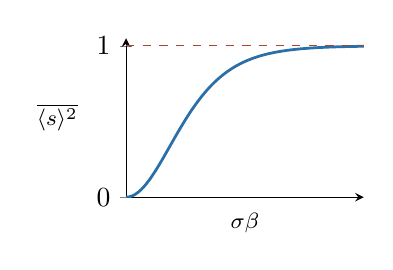
\begin{tikzpicture}
\begin{axis}[
  width=4.6cm,height=3.6cm,
  xlabel={\footnotesize $\sigma\beta$},
  ylabel={\footnotesize $\dbar{\langle s\rangle^2}$},
  xmin=0,xmax=4,ymin=0,ymax=1.05,
  xtick=\empty, ytick={0,1}, 
  axis lines=left, every axis plot/.append style={line width=1pt},
  ylabel style={rotate=-90}]
  \addplot[accent,domain=0:4,samples=80]{tanh(0.9*x)^2};
  \draw[spindown,dashed] (axis cs:0,1)--(axis cs:4,1);
\end{axis}
\end{tikzpicture}\\[2pt]
\footnotesize The single-neuron learning crossover: output determinacy
rises from $0$ (undetermined) toward $1$ (data-locked) as the signal
$\sigma\beta$ grows.}

\newthought{The crossover} between these regimes is the toy precursor of a
learning transition. As $\sigma\beta$ increases,
\[
  \sigma\beta\to0:\ \dbar{\ln Z}\to\ln 2 \ (\text{1 bit free}),
  \qquad
  \sigma\beta\to\infty:\ \dbar{\ln Z}\to \sigma\beta\sqrt{\tfrac{2}{\pi}}
  \ (\text{locked to data}),
\]
using $\ln(2\cosh x)\to|x|$ and $\dbar{|z|}=\sqrt{2/\pi}$. Here the
crossover is perfectly smooth. In a network of many coupled spins it will
\emph{sharpen into a genuine phase transition}---the subject of
Chapter~5.

%---------------------------------------------------------------------
\section{What this chapter established}

The logical skeleton, which survives intact into real spin glasses and
machine-learning calculations, is:
\begin{enumerate}
\item We want $\dbar{\ln Z}$; it is intractable because the logarithm does
  not factorise over disorder.
\item Replace it via $\ln Z=\lim_{n\to0}(Z^n-1)/n$, so we instead need
  $\dbar{Z^n}$.
\item For integer $n$, $Z^n$ is $n$ replicas sharing the disorder;
  averaging is a tractable Gaussian integral.
\item Disorder averaging \emph{couples} the replicas, producing
  $s^a s^b$---whose many-spin analogue is the overlap $q_{ab}$.
\item Evaluate $\dbar{Z^n}$ as a function of $n$, continue to real $n$,
  and take $n\to 0$.
\end{enumerate}

\newthought{What made this case easy} was the absence of two ingredients.
There was no thermodynamic limit ($N\to\infty$), so no saddle point: the
disorder average was an exact finite integral. And the overlap $s^a s^b$
was a single number, not a matrix we had to solve for. Restore both---many
coupled spins, and a matrix-valued overlap $q_{ab}$ determined
self-consistently---and the replica method begins to do work that nothing
else can: it predicts the storage capacity of a memory, the shape of a
learning curve, and the sharp transitions between learnable and
unlearnable regimes. That is Chapter~6.

\end{document}
